\documentclass[12pt,a4paper]{article}
\usepackage[utf8]{inputenc}
\usepackage[vietnamese]{babel}
\usepackage{amsmath}
\usepackage{amsfonts}
\usepackage{amssymb}
\usepackage{makeidx}
\usepackage{graphicx}
\usepackage{amsmath,amsfonts,amssymb,amsthm}
\usepackage{algorithm}
\usepackage{algorithmic}
\usepackage[left=2cm,right=2cm,top=2cm,bottom=2cm]{geometry}
\begin{document}
\begin{algorithm}[H]
\caption{Chuyển từ NFA sang DFA}
\begin{algorithmic} 
\STATE \textbf{Input} (NFA) $M = \{Q, A, \delta, q_0, F\}$
\STATE \textbf{Output} (DFA) $M' = \{Q', A, \delta', q_0', F'\}$
\STATE Khởi tạo $Q' = \{q_0\}, F' = \emptyset$
\WHILE{$\exists \delta'(q_x, a)$ chưa xác định với $q_x \in Q', a \in A$}
\STATE Chọn $q_x' \in Q', a \in A$ sao cho $\delta'(q_x', a)$ chưa xác định
\STATE Gán $q_{xa} = \delta'(q_x, a) = \{q \in Q | \delta(q', a) = q, q' \in q_x'\}$
\IF{$q_{xa} \notin Q'$}
\STATE $Q' = Q' \cup q_{xa}$
\ENDIF
\IF{$q_{xa} \cap F \ne \emptyset$}
\STATE $F' = F' \cup q_{xa}$
\ENDIF
\ENDWHILE
\end{algorithmic}
\end{algorithm}
%----------------------------------------------------------------------------------
--------------------------------------------------------------------------------\\

\textbf{Bổ đề Arden}: Với $X, A, B$ là các xâu kí tự, phương trình $X = A.X + B$ có nghiệm duy nhất là $X = A^*.B$\\
Xét DFA hoặc NFA $M = \{Q, A, \delta, q_0, F\}$ có $n$ trạng thái, với mỗi trạng thái $q_i$ ta đưa ra một phương trình có dạng:
\[\qquad \displaystyle Q_i = \bigcup\limits_{q_i \overset{a}{\to} q_j} a.Q_j + \begin{cases} \{\varepsilon\} &,\ q_i \in F \\ \emptyset &, \text{ngược lại}\end{cases}\]
Ta thấy ta luôn có thể đưa về hệ phương trình như sau:
\[X_i = B_i + A_{i,1}X_1 + … + A_{i,n}X_n \text{ trong đó } i = 1, 2, ..., n\]
Ta có thể giải hệ này để tìm ra được biểu thức chính quy tương ứng.\\
Xét với $i=n$:
\[X_n = B_n + A_{n,1}X_1 + … + A_{n,n}X_n\]
Theo bổ đề Arden, phương trình trên sẽ có nghiệm là 
\[X_n = A_{n,n}^* (B_n + A_{n,1}X_1 + … + A_{n,n-1}X_{n-1})\]
Bằng cách đặt $B'_n = A_{n,n}^* B_n$ và $A'_{n,i}=A_{n,n}^*A_{n,i}$, ta được:
\[X_n = B'_n + A'_{n,1}X_1 + … + A'_{n,n-1}X_{n-1}\]
Do đó, ta có thể bỏ $X_n$ khỏi các phương trình của hệ bằng cách đặt:
\[B'_i = B_i + A_{i,n}B'_n\]
\[A'_{i,j} = A_{i,j} + A_{i,n}A'_{n,j}\]
với $i, j < n$.\\
Làm như vậy cho đến khi $i=1$, ta sẽ được phương trình có dạng:
\[X_1 = B_1'\]
Đây chính là biểu thức chính quy cần tìm.
\begin{algorithm}[H]
\caption{Tìm ngôn ngữ chính quy được đón nhận bởi FA}
\begin{algorithmic} 
\STATE \textbf{Input} DFA hoặc NFA $M = \{Q, A, \delta, q_0, F\}$
\STATE \textbf{Output} Biểu thức chính quy biểu diễn ngôn ngữ chính quy tương ứng
\STATE Khởi tạo mảng $B$ gồm $n$ phần tử, $B[i] = \epsilon$ nếu $q_i \in F$, ngược lại $B[i] = \emptyset$.
\STATE Khởi tạo mảng $A$ kích thước $n \times n$, $A[i, j] = \emptyset$ với mọi $i, j \in \{0, n-1\}$
\STATE Nếu $\delta{q_i, a} = q_j$ thì đặt $A[i, j] = a$
\FOR{$m=n$ to $1$}
\STATE Gán $B[m] = (A[m, m])^*.B[m]$
\FOR{$j=1$ to $m$}
\STATE Gán $A[m, j] = (A[m, m])^*.A[m, j]$
\ENDFOR
\FOR{$i=1$ to $m$}
\STATE Gán $B[i] = B[i] + A[i, m].B[m]$
\FOR{$j=1$ to $m$}
\STATE Gán $A[i, j] = A[i, j] + A[i, m].A[m, j]$
\ENDFOR
\ENDFOR
\ENDFOR
\end{algorithmic}
\end{algorithm}
%----------------------------------------------------------------------------------
--------------------------------------------------------------------------------\\

Ta sẽ xây dựng NFA như sau:\\
- Kí tự rỗng:
\begin{center}
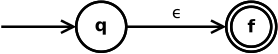
\includegraphics[scale=0.7]{empty.png}
\end{center}
- Kí tự $a \in A$:
\begin{center}
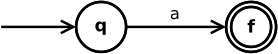
\includegraphics[scale=0.7]{symbol.png}
\end{center}
- Phép hợp $s+t$:
\begin{center}
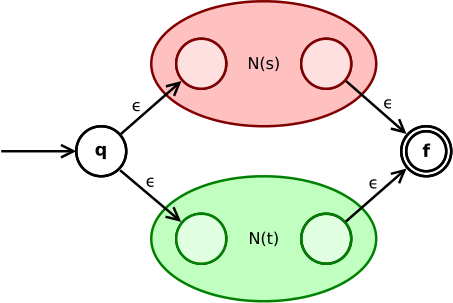
\includegraphics[scale=0.6]{union.png}
\end{center}
- Phép tích ghép $s.t$:
\begin{center}
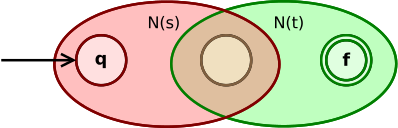
\includegraphics[scale=0.6]{concac.png}
\end{center}
- Phép $s^*$:
\begin{center}
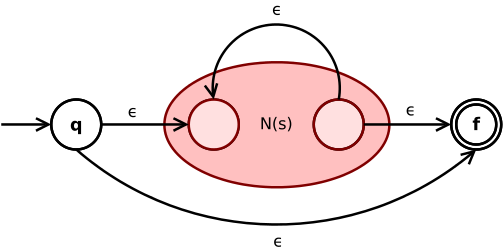
\includegraphics[scale=0.6]{star.png}
\end{center}

\begin{algorithm}[H]
\caption{Xây dựng FA đoán nhận ngôn ngữ chính quy}
\begin{algorithmic} 
\STATE \textbf{Input} Biểu thức chính quy $s$ biểu diễn ngôn ngữ chính quy
\STATE \textbf{Output} FA $M = \{Q, A, \delta, q_0, F\}$
\STATE Duyệt biểu thức chính quy, thực hiện xây dựng NFA như mô tả bên trên.
\STATE Từ NFA trên ta tiếp tục thực hiện chuyển từ NFA sang DFA, tối tiểu hóa nếu cần.
\end{algorithmic}
\end{algorithm}
%----------------------------------------------------------------------------------
--------------------------------------------------------------------------------\\
\begin{algorithm}[H]
\caption{Chuyển từ văn phạm tuyến tính trái sang văn phạm tuyến tính phải}
\begin{algorithmic} 
\STATE \textbf{Input} Văn phạm tuyến tính trái $G_T = \{V_T, V_N, S, P\}$
\STATE \textbf{Output} Văn phạm tuyến tính phải $G_P = \{V_T', V_N', S', P'\}$
\IF{tồn tại luật có dạng $S \rightarrow Sw$ với $w \in V_T*$}
\STATE Thêm vào $V_N$ $S_0$, thêm luật $S_0 \rightarrow S$ vào $P$, đặt $S = S_0$.
\ENDIF
\STATE Khởi tạo $V_T' = V_T, V_N' = V_N, P' = \emptyset, S' = S$
\FOR{\textbf{each} luật $p \in P$}
\IF{luật có dạng $S \rightarrow p$}
\STATE Thêm luật đó vào $P'$
\ELSIF{luật có dạng $A \rightarrow w$}
\STATE Thêm luật $S \rightarrow wA$ vào $P'$
\ELSIF{luật có dạng $B \rightarrow Aw$}
\STATE Thêm luật $A \rightarrow wB$ vào $P'$
\ELSIF{luật có dạng $S \rightarrow Aw$}
\STATE Thêm luật $A \rightarrow w$ vào $P'$
\ENDIF
\ENDFOR
\end{algorithmic}
\end{algorithm}

%----------------------------------------------------------------------------------
--------------------------------------------------------------------------------\\
\begin{algorithm}[H]
\caption{Xây dựng NFA từ văn phạm chính quy}
\begin{algorithmic} 
\STATE \textbf{Input} Văn phạm chính quy $G = \{V_T, V_N, S, P\}$
\STATE \textbf{Output} NFA $M = \{Q, A, \delta, q_0, F\}$ tương ứng với văn phạm đã cho.
\IF{Văn phạm $G$ là tuyến tính trái}
\STATE Chuyển $G$ về dạng tuyến tính phải
\ENDIF
\STATE Khởi tạo $A = V_T$
\FOR{\textbf{each} $v \in V_N$}
\STATE Tạo trạng thái $q_{v}$ mới tương ứng.
\STATE Thêm $q_{v}$ vào $Q$.
\ENDFOR
\STATE Gán $q_0 = q_S$
\STATE Thêm trạng thái $q_\epsilon$ vào $Q$, đặt $F = \{q_\epsilon\}$
\FOR{\textbf{each} luật $p \in P$}
\STATE Với $p = A \rightarrow wB$ trong đó $A \in V_N, B \in V_N \cup \{\epsilon\}, w \in V_T^*, w = w_1.w_2...w_n$
\STATE Thêm các trạng thái $q_{pw_1}, q_{pw_2}, ..., q_{pw_{n-1}}$ vào $Q$.
\STATE Gán $\delta(q_{pw_i}, w_{i+1}) = q_{pw_{i+1}}$ với $i=1,...,n-2$.
\STATE Gán $\delta(q_A, w_1) = q_{pw_1}$, $\delta(q_{pw_{n-1}}, w_n) = q_B$.
\ENDFOR
\end{algorithmic}
\end{algorithm}

%----------------------------------------------------------------------------------
--------------------------------------------------------------------------------\\
\begin{algorithm}[H]
\caption{Chuyển từ NFA sang văn phạm tuyến tính phải}
\begin{algorithmic} 
\STATE \textbf{Input} NFA $M = \{Q, A, \delta, q_0, F\}$
\STATE \textbf{Output} Văn phạm tuyến tính phải $G = \{V_T, V_N, S, P\}$ tương ứng với NFA đã cho.
\STATE Khởi tạo $V_T = A, V_N = Q, S = q_0$
\FOR{\textbf{each} $q_i \in Q$}
\FOR{\textbf{each} $a \in A$}
\FOR{\textbf{each} $q_j \in \delta(q_i, a)$}
\STATE Thêm luật $q_i \rightarrow aq_j$ vào $P$
\ENDFOR
\ENDFOR
\ENDFOR
\FOR{\textbf{each} $q_i \in F$}
\STATE Thêm luật $q_i \rightarrow \epsilon$ vào $P$
\ENDFOR
\end{algorithmic}
\end{algorithm}

%----------------------------------------------------------------------------------
--------------------------------------------------------------------------------\\
\begin{algorithm}[H]
\caption{Tìm ngôn ngữ chính quy được sinh bởi văn phạm chính quy}
\begin{algorithmic} 
\STATE \textbf{Input} Văn phạm chính quy $G = \{V_T, V_N, S, P\}$
\STATE \textbf{Output} Ngôn ngữ chính quy ứng với văn phạm đã cho
\STATE Chuyển văn phạm chính quy về NFA
\STATE Từ NFA thực hiện chuyển về ngôn ngữ chính quy.
\end{algorithmic}
\end{algorithm}

%----------------------------------------------------------------------------------
--------------------------------------------------------------------------------\\
\begin{algorithm}[H]
\caption{Tìm ngôn ngữ chính quy sinh ra bởi văn phạm tuyến tính phải}
\begin{algorithmic} 
\STATE \textbf{Input} Ngôn ngữ chính quy $L$
\STATE \textbf{Output} Văn phạm chính quy $G = \{V_T, V_N, S, P\}$ ứng với biểu thức chính quy đã cho
\STATE Tìm NFA đoán nhận ngôn ngữ chính quy $L$
\STATE Từ NFA thực hiện chuyển về văn phạm tuyến tính phải.
\end{algorithmic}
\end{algorithm}

%----------------------------------------------------------------------------------
--------------------------------------------------------------------------------\\
\section{Mã Hamming}
\subsection{Giới thiệu}
Mã Hamming là một mã sửa lỗi, được đặt tên theo người phát minh ra nó, Richard Hamming. Mã Hamming có thể phát hiện một bit hoặc hai bit lỗi. Mã Hamming còn có thể sửa các lỗi do một bit bị sai gây ra.
\subsection{Lịch sử phát triển}
\subsubsection{Mã chẵn lẻ}

Trước mã hamming, người ta sử dụng mã chẵn lẻ. Mã chẵn lẻ thêm một bit vào trong dữ liệu, và bit này cho biết số lượng bit có giá trị $1$ của đoạn dữ liệu nằm trước là một số chẵn hay một số lẻ. Nếu một bit bị thay đổi trong quá trình truyền dữ liệu, giá trị chẵn lẻ trong thông điệp sẽ thay đổi và do đó có thể phát hiện được lỗi. Theo quy ước chung, bit kiểm tra có giá trị bằng $1$ nếu số lượng bit có giá trị một trong dữ liệu là một số lẻ, và giá trị của bit kiểm tra bằng $0$ nếu số lượng bit có giá trị một trong dữ liệu là một số chẵn. Nói cách khác, nếu đoạn dữ liệu và bit kiểm tra được gộp lại cùng với nhau, số lượng bit có giá trị bằng $1$ luôn luôn là một số chẵn.\\

Việc kiểm tra dùng mã chẵn lẻ là một việc không được chắc chắn cho lắm, vì nếu số bit bị thay đổi là một số chẵn thì mã này không phát hiện được lỗi. Hơn nữa, mã chẵn lẻ không biết đươck bit nào là bit lỗi, kể cả khi nó phát hiện có lỗi xảy ra. Toàn bộ dữ liệu đã nhận được phải bỏ đi và truyền lại từ đầu. 
\subsubsection{Mã hai-trong-năm}


Trong những năm của thập niên kỷ 1940, Bell có sử dụng một mã hiệu phức tạp hơn một chút, gọi là mã hai-trong-năm (two-out-of-five code). Mã này đảm bảo mỗi một khối 5 bit (còn được gọi là khối-5) có chính xác hai bit có giá trị bằng 1. Máy tính có thể nhận ra là dữ liệu nhập vào có lỗi nếu trong một khối $5$ bit không $2$ bit có giá trị bằng $1$. Tuy thế, mã hai-trong-năm cũng chỉ có thể phát hiện được một đơn vị bit mà thôi; nếu trong cùng một khối, một bit bị lộn ngược thành giá trị $1$, và một bit khác bị lộn ngược thành giá trị $0$, quy luật hai-trong-năm vẫn cho một giá trị đúng (remained true), và do đó nó không phát hiện là có lỗi xảy ra.
\subsubsection{Tái diễn dữ liệu}



Một mã nữa được dùng trong thời gian này là mã hoạt động bằng cách nhắc đi nhắc lại bit dữ liệu vài lần (tái diễn bit được truyền) để đảm bảo bit dữ liệu được truyền, truyền đến nơi nhận trọn vẹn. Chẳng hạn, nếu bit dữ liệu cần được truyền có giá trị bằng 1, một mã tái diễn $n=3$ sẽ cho truyền gửi giá trị "$111$". Nếu ba bit nhận được không giống nhau, thì hiện trạng này báo cho ta biết rằng, lỗi trong truyền thông đã xảy ra. Nếu kênh truyền không bị nhiễu, tương đối đảm bảo, thì với hầu hết các lần truyền, trong nhóm ba bit được gửi, chỉ có một bit là bị thay đổi. Do đó các nhóm $001, 010$, và $100$ đều tương đương cho một bit có giá trị $0$, và các nhóm $110$, $101$, và $011$ đều tương đương cho một bit có giá trị $1$ - lưu ý số lượng bit có giá trị $0$ trong các nhóm được coi là có giá trị $0$, là đa số so với tổng số bit trong nhóm, hay $2$ trong $3$ bit, tương đương như vậy, các nhóm được coi là giá trị $1$ có số lượng bit bằng $1$ nhiều hơn là các bit có giá trị $0$ trong nhóm - chẳng khác gì việc các nhóm bit được đối xử như là "các phiếu bầu" cho bit dữ liệu gốc vậy. Một mã có khả năng tái dựng lại thông điệp gốc trong một môi trường nhiễu lỗi được gọi là mã "sửa lỗi" (error-correcting code).

Tuy nhiên, những mã này không thể sửa tất cả các lỗi một cách đúng đắn hoàn toàn. Chẳng hạn chúng ta có một ví dụ sau: nếu một kênh truyền đảo ngược hai bit và do đó máy nhận thu được giá trị "$001$", hệ thống máy sẽ phát hiện là có lỗi xảy ra, song lại kết luận rằng bit dữ liệu gốc là bit có giá trị bằng $0$. Đây là một kết luận sai lầm. Nếu chúng ta tăng số lần các bit được nhắc lại lên $4$ lần, chúng ta có thể phát hiện tất cả các trường hợp khi $2$ bit bị lỗi, song chúng ta không thể sửa chữa chúng được (số phiếu bầu "hòa"); với số lần nhắc lại là $5$ lần, chúng ta có thể sửa chữa tất cả các trường hợp $2$ bit bị lỗi, song không thể phát hiện ra các trường hợp $3$ bit bị lỗi.

Nói chung, mã tái diễn là một mã hết sức không hiệu quả, giảm công suất xuống $3$ lần so với trường hợp đầu tiên trong ví dụ trên của chúng ta, và công suất làm việc giảm xuống một cách nhanh chóng nếu chúng ta tăng số lần các bit được nhắc lại với mục đích để sửa nhiều lỗi hơn.
\subsection{Xây dựng mã Hamming}
Hamming nghiên cứu các kế hoạch mã hóa hiện có, rồi tổng quát hóa khái niệm. Ông xây dựng một danh mục để diễn tả hệ thống máy, bao gồm cả số lượng bit dùng cho dữ liệu và các bit sửa lỗi trong một khối. Chẳng hạn, nếu một từ dữ liệu có 8 bit chỉ gồm 7 bit chứa dữ liệu và phải thêm 1 bit sửa lỗi vào, ông diễn tả phương pháp này là mã $(8, 7)$. Như vậy mã tái diễn sẽ được gọi là mã $(3, 1)$. Ông đưa ra khái niệm "tỷ lệ thông tin", được tính bằng lấy con số thứ hai chia cho con số thứ nhất. Ví dụ, với mã tái diễn, tỷ lệ thông tin sẽ là $\frac{1}{3}$.\\

Hamming còn phát hiện ra nan đề với việc đảo giá trị của hai hoặc hơn hai bit nữa, và miêu tả nó là "khoảng cách" (distance) (hiện nay nó được gọi là khoảng cách Hamming (Hamming distance) - theo cái tên của ông). Mã chẵn lẻ có khoảng cách bằng $2$, vì nếu có $2$ bit bị đảo ngược thì lỗi trong truyền thông trở nên vô hình, không phát hiện được. Mã tái diễn $(3,1$) có khoảng cách là $3$, vì $3$ bit, trong cùng một bộ ba, phải bị đổi ngược trước khi chúng ta được một từ mã khác. Mã tái diễn $(4,1)$ (mỗi bit được nhắc lại $4$ lần) có khoảng cách bằng $4$, nên nếu $2$ bit trong cùng một nhóm bị đảo ngược thì lỗi đảo ngược này sẽ đi thoát mà không bị phát hiện.\\

Cùng một lúc, Hamming quan tâm đến hai vấn đề; tăng khoảng cách và đồng thời tăng tỷ lệ thông tin lên, càng nhiều càng tốt. Trong những năm thuộc niên kỷ 1940, ông đã xây dựng một số kế hoạch mã hóa. Những kế hoạch này đều dựa trên những mã đang tồn tại song được nâng cấp và tiến bộ một cách sâu sắc. Bí quyết chìa khóa cho tất cả các hệ thống của ông là việc cho các bit chẵn lẻ gối lên nhau (overlap), sao cho chúng có khả năng tự kiểm tra lẫn nhau trong khi cùng kiểm tra được dữ liệu nữa.

Thuật toán cho việc xây dựng mã Hamming như sau:
\begin{itemize}
\item Tất cả các bit ở vị trí là các số mũ của 2 được dùng làm bit chẵn lẻ. (các vị trí như $1$, $2$, $4$, $8$, ...)
\item Tất cả các vị trí bit khác được dùng cho dữ liệu sẽ được mã hóa.
\item Mỗi bit chẵn lẻ đếm số lượng bit $1$ cho một số bit trong từ mã. Vị trí của bit chẵn lẻ quyết định chuỗi các bit mà nó kiểm tra.
\begin{itemize}
     \item Bit chẵn lẻ ở vị trí $1$ kiểm tra các bit có $1$ ở cuối trong vị trí được viết dưới dạng nhị phân (1=1, 3=11, 5=101, 7=111, ...) 
     \item Bit chẵn lẻ ở vị trí $2$ kiểm tra các bit có $1$ ở thứ hai trong vị trí được viết dưới dạng nhị phân (2=10, 3=11, 6=110, 7=111, ...)
     \item Bit chẵn lẻ ở vị trí $4$ kiểm tra các bit có $1$ ở thứ ba trong vị trí được viết dưới dạng nhị phân (4-7, 12-15, 20-23, ...)
     \item Bit chẵn lẻ ở vị trí $8$ kiểm tra các bit có $1$ ở thứ tư trong vị trí được viết dưới dạng nhị phân (8-15, 24-31, 40-47, ...)
\end{itemize}

\end{itemize}

\subsection{Ví dụ mã Hamming (11, 7)}
Lấy ví dụ chúng ta có một từ dữ liệu dài 7 bit với giá trị là "$0110101$". Để chứng minh phương pháp các mã Hamming được tính toán và được sử dụng để kiểm tra lỗi, xin xem bảng liệt kê dưới đây. Chữ d (data) được dùng để biểu thị các bit dữ liệu và chữ p (parity) để biểu thị các bit chẵn lẻ (parity bits).
\begin{center}
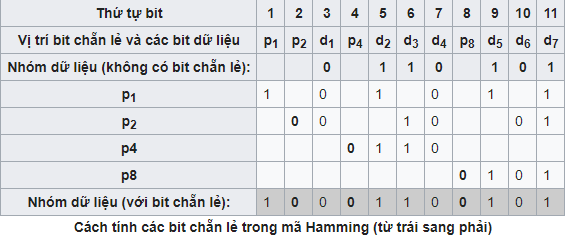
\includegraphics[scale=0.8]{bang1.png}
\end{center}
Dữ liệu mới - bao gồm các bit chẵn lẻ - bây giờ là "$10001100101$". Nếu chúng ta thử cho rằng bit cuối cùng bị sai từ 1 sang 0. Nhóm dữ liệu mới sẽ là "$10001100100$"; Dưới đây, chúng ta sẽ phân tích quy luật kiến tạo mã Hamming bằng cách cho bit chẵn lẻ giá trị 1 khi kết quả kiểm tra dùng quy luật số chẵn bị sai.
\begin{center}
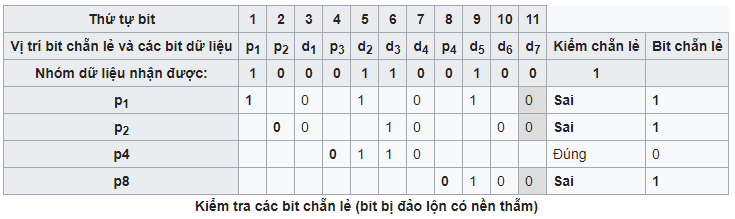
\includegraphics[scale=0.8]{bang2.png}
\end{center}
Bước cuối cùng là định giá trị của các bit chẵn lẻ (nên nhớ bit nằm dưới cùng được viết về bên phải - viết ngược lại từ dưới lên trên). Giá trị số nguyên của các bit chẵn lẻ là 11, và như vậy có nghĩa là bit thứ 11 trong nhóm dữ liệu (data word) - bao gồm cả các bit chẵn lẻ - là bit có giá trị không đúng, và bit này cần phải đổi ngược lại.
\begin{center}
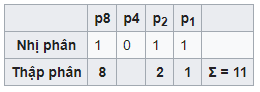
\includegraphics[scale=0.8]{bang3.png}
\end{center}
Bằng việc sửa lỗi và bỏ đi phần mã Hamming, chúng ta lấy được phần dữ liệu gốc với giá trị là $0110101$.\\

Lưu ý, các bit chẵn lẻ không kiểm tra được lẫn nhau, nếu chỉ một bit chẵn lẻ bị sai thôi, trong khi tất cả các bit khác là đúng, thì chỉ có bit chẵn lẻ nói đến là sai mà thôi và không phải là các bit nó kiểm tra (not any bit it checks).\\

Cuối cùng, giả sử có hai bit biến đổi, tại vị trí $x$ và $y$. Nếu $x$ và $y$ có cùng một bit tại vị trí $2^k$ trong đại diện nhị phân của chúng, thì bit chẵn lẻ tương ứng với vị trí đấy kiểm tra cả hai bit, và do đó sẽ giữ nguyên giá trị, không thay đổi. Song một số bit chẵn lẻ nào đấy nhất định phải bị thay đổi, vì $x \ne y$, và do đó hai bit tương ứng nào đó có giá trị $x$ và $y$ khác nhau. Do vậy, mã Hamming phát hiện tất cả các lỗi do hai bit bị thay đổi — song nó không phân biệt được chúng với các lỗi do 1 bit bị thay đổi.



\end{document}




